\input{Inhalt/05/00-tikzDefs.tex}

\begin{document}
\title{Übungsblatt~5}
\subtitle{Schlüssel -- B-Baum, B*-Baum}
\maketitle

\begin{note}
Für einige der Übungen des Blattes kann \url{http://faui6g.informatik.uni-erlangen.de/} verwendet werden.
\end{note}

\section*{Lernziele}
\begin{itemize}
	\item Auftretende Probleme bei nicht isolierten Transaktionen
	\item Möglichkeiten, diese Probleme zu erkennen und zu vermeiden
	\item Möglichkeiten zur Recovery unter Verwendung von Logs
\end{itemize}


\section*{Literatur}
\HaerderNintyNine{14}

\ElmasriFive{18, insbes. 18.1}

\GarciaMolinaFirst{18}

\BerensonNintyFive

\section{Fragen zur Vorlesung}

\begin{enumerate}[a)]
	\item Welche möglichen Probleme bei der gleichzeitigen Ausführung von Transaktionen haben Sie in der Vorlesung kennengelernt?

\begin{solution}
\begin{itemize}
	\item Verlorengegangene Änderung (Dirty Write, Lost Update)
	\item Lesen nicht freigegebener Änderungen (Dirty Read)
	\item Inkonsistente Analyse (Non-Repeatable Read)
	\item Phantom-Problem
\end{itemize}
Für die Anomalien im Mehrbenutzerbetrieb gibt man bestimmte Abläufe,
d.\,h.\ Ausführungsreihenfolgen von Operationen verschiedener Transaktionen,
als Muster an.
Beinhaltet ein Ablauf das Muster einer Anomalie,
so sagt man:
Die Anomalie tritt in diesem Ablauf auf.

Leider ist die Definition der Anomalie-Muster umstritten.
Das zeigt sich u.\,a.\ daran, dass viele reale Systeme (z.\,B.\ Oracle, PostgreSQL) nach unserer Definition nicht serialisierbar (und damit möglicherweise nicht korrekt) arbeiten, da sie eine andere Definition verwenden.
Für eine tiefere Beschäftigung mit dieser Tatsache sei der Artikel von Berenson et al.\ empfohlen.
Für diese Veranstaltung ist das aber nicht notwendig.

Da aber eine Definition von Anomalie-Abläufen nötig ist, um über Anomalien sprechen zu können, verwenden wir die Definitionen aus dem Artikel von Berenson et al. (Vorlesungsfolie~\AnomalieDef):

\paragraph{\color{solutioncolor}Dirty Write}
$w_1[x] \ldots w_2[x] \ldots
((c_1 \textrm{ oder } a_1) \textrm{ und } (c_2 \textrm{ oder } a_2)$
in beliebiger Reihenfolge)

Zwei Transaktionen schreiben überschneidend dasselbe Datenelement,
wodurch Inkonsistenzen entstehen können
und das Rücksetzen von Transaktionen erschwert wird.

\paragraph{\color{solutioncolor}Dirty Read}
$w_1[x] \ldots r_2[x] \ldots
((c_1 \textrm{ oder } a_1) \textrm{ und } (c_2 \textrm{ oder } a_2)$
in beliebiger Reihenfolge)

Transaktion~2 hat Daten gelesen, die inkonsistent zu anderen Daten sein können und die eventuell "`nie existiert haben"', da Transaktion~1 abgebrochen werden könnte und damit alle ihre Änderungen rückgängig gemacht werden.

\paragraph{\color{solutioncolor}Non-Repeatable Read}
$r_1[x] \ldots w_2[x] \ldots
((c_1 \textrm{ oder } a_1) \textrm{ und } (c_2 \textrm{ oder } a_2)$
in beliebiger Reihenfolge)

Transaktion~1 sieht, wenn sie erneut liest, einen anderen Wert als zuvor. Dadurch kann es zu inkonsistenten Analysen kommen.

\paragraph{\color{solutioncolor}Phantom-Problem}
$r_1[P] \ldots w_2[y \textrm{ in } P] \ldots
((c_1 \textrm{ oder } a_1) \textrm{ und } (c_2 \textrm{ oder } a_2)$
in beliebiger Reihenfolge);
$P$ steht hier für die Menge der Datenobjekte, die ein Prädikat erfüllen.

Nachdem Transaktion~1 $P$ liest, verändert Transaktion~2 diese Menge durch Einfügen eines geeigneten Tupels, wodurch inkonsistente Analysen entstehen können.
\end{solution}

\begin{note}
Eine Anomalie liegt unabhängig davon vor, ob die Transaktionen mit Abort oder Commit enden, und unabhängig von der Reihenfolge des Endes. Damit die Anomalie vorliegt, dürfen beide Transaktionen aber erst \emph{nach} den anderen Operationen (z.\,B.\ $(r_1[x] w_2[x])$ bei Non-Repeatable Read) enden. Der Ablauf $(r_1[x] c_1[x] w_2[x] a_2[x])$ ist also kein Non-Repeatable Read, der Ablauf $(r_1[x] w_2[x] c_1[x] a_2[x])$ schon.

Das Datenbanksystem kann nicht prüfen, ob eine Anomalie zu einem Problem wird oder nicht, da es nicht weiß, was das Anwendungsprogramm mit den Daten macht. Sobald eine Anomalie vorliegt, besteht aber die Möglichkeit, dass ein Problem, also ein anderes Ergebnis als bei einem seriellen Ablauf, entsteht. Deshalb muss das Datenbanksystem Abläufe mit Anomalien verhindern. Umgekehrt betrachtet muss also in jedem Ablauf, der zu einem Problem führt, eine Anomalie vorliegen.

Beispiel für ein Non-Repeatable Read (und dafür, warum nach Berenson et al.\ kein zweites $(r_1[x])$ gefordert wird), direkt aus Berenson et al.:

x und y seien zwei Kontostände, T1 möchte die Summe der beiden Kontostände ermitteln, T2 nimmt eine Umbuchung von 40 von x auf y vor.

$(r_1[x=50] r_2[x=50] w_2[x=10] r_2[y=50] w_2[y=90] c_2 r_1[y=90] c_1)$

T1 sieht eine Summe von 140 statt der korrekten 100. Die Anomalie ist ein Non-Repeatable Read aufgrund von $(r_1[x=50] \ldots w_2[x=10] \ldots c_2 \ldots c_1)$
Würde Non-Repeatable Read ein zweites $(r_1[x])$ erfordern, würde in dem Ablauf keine Anomalie auftreten.

Zentraler Punkt in Berenson et al., \emph{A Critique of ANSI SQL Isolation Levels} ist folgender:
Einige Anomalien werden durch den SQL-Standard wie folgt definiert:
\begin{enumerate}[i)]
  \item P1 ("`Dirty read"'): SQL-transaction $T_1$ modifies a row. SQL-transaction $T_2$ then reads that row before $T_1$ performs a COMMIT. If $T_1$ then performs a ROLLBACK, $T_2$ will have read a row that was never committed and that may thus be considered to have never existed.

  \item P2 ("`Non-repeatable read"'): SQL-transaction $T_1$ reads a row. SQL-transaction $T_2$ then modifies or deletes that row and performs a COMMIT. If $T_1$ then attempts to reread the row, it may receive the modified value or discover that the row has been deleted.

  \item P3 ("`Phantom"'): SQL-transaction $T_1$ reads the set of rows N that satisfy some $<$search condition$>$. SQL-transaction $T_2$ then executes SQL-statements that generate one or more rows that satisfy the $<$search condition$>$ used by SQL-transaction $T_1$. If SQL-transaction $T_1$ then repeats the initial read with the same $<$search condition$>$, it obtains a different collection of rows.
\end{enumerate}

Dabei ist nun ungeklärt, ob der jeweilige "`If"'-Teil zur Definition der Anomalie gehört oder nur eine Erklärung dessen darstellt, was bei Auftreten der Anomalie passieren kann. Konkret: Muss $T_1$ ein ROLLBACK durchführen, damit ein Dirty Read vorliegt? Oder liegt der bereits durch $w_1(x) r_1(x)$ vor und der "`If $T_1$ \ldots "'-Satz erläutert nur, warum das schlimm sein kann? Genau das ist umstritten. Aber für uns gelten die Definitionen, die oben angegeben sind.
\end{note}

\item Definieren Sie den Begriff "`Serialisierbarkeit"'.

\begin{solution}
Direkt aus den Vorlesungsfolien:
Ein Schedule von Transaktionen ist serialisierbar, wenn er zu irgendeinem seriellen Ablauf der in ihm enthaltenen Transaktionen äquivalent ist.
\end{solution}


\item Seien $T_i$ und $T_j$ beliebige Transaktionen und $H$ und $G$ zwei
  dazugehörige Abläufe. Markieren Sie die Bedingungen, die für alle
  Operationen auf einem beliebigen Datenobjekt $A$ gelten müssen, damit
  zwei Abläufe nach der Definition der Vorlesung "`äquivalent"' sind.
  \nt{Studierende darauf Hinweisen, dass in der Klausur ausgefüllt und nicht gekreuzt wird. Korrekturen mit Korrekturband.}

  \begin{itemize}
    \itemmc   \hspace*{0.45em} $r_i[A] <_H r_j[A] \Leftrightarrow r_i[A] <_G r_j[A]$
    \itemmcsol \hspace*{0.45em} $r_i[A] <_H w_j[A] \Leftrightarrow r_i[A] <_G w_j[A]$
    \itemmcsol \hspace*{0.45em} $w_i[A] <_H r_j[A] \Leftrightarrow w_i[A] <_G r_j[A]$
    \itemmcsol \hspace*{0.45em} $w_i[A] <_H w_j[A] \Leftrightarrow w_i[A] <_G w_j[A]$
  \end{itemize}

\item Geben Sie eine Möglichkeit an, Serialisierbarkeit zu gewährleisten.

\begin{solution}
Serialisierung oder Sperren.
Abhängigkeitsgraphen zählen nicht, da sie zur Prüfung dienen.
Sicherstellen muss man das dann noch auf anderem Wege.
\end{solution}

\begin{note}
Aus didaktischen Gründen lassen wir den Unterschied zwischen Konflikt-Serialisierbarkeit und anderen Serialisierbarkeitsarten aus.
Ersteres ist ein stärkeres Kriterium und wird sowohl durch Abhängigkeitsgraphen als auch durch 2PL gewährleistet.
Wir verbieten also einige Abläufe, die wir eigentlich erlauben könnten.
Grund: Konflikt-Serialisierbarkeit ist leichter zu prüfen.
\end{note}

\end{enumerate}


\section{Fragen zur Vorlesung}
\begin{enumerate}[a)]
	\item Was ist der Vorteil eines B-Baums gegenüber binären Suchbäumen?

	\begin{solution}
	Größerer Fan-Out (Verzweigungsgrad) $\rightarrow$ Grundidee: Blockzugriff ist teuer, also weniger davon machen.

	Das ist auch der Grund, warum ein Knoten gerade so groß wie ein Block ist. Ein Knoten ist die Einheit, in der wir nach der nächsten Verzweigung suchen. Sie sollte komplett zur Verfügung stehen und keine zwischenzeitlichen I/Os verursachen.
	\end{solution}


	\item Was sind die charakteristischen Eigenschaften eines B-Baums?

	\begin{solution}
	Perfekt balanciert (alle Pfade von der Wurzel zu einem Blatt sind gleich lang), jeder innere Knoten hat zwischen $k+1$ und $2k+1$ Nachfolger. Jeder Knoten außer der Wurzel ist mindestens zur Hälfte gefüllt. Die Wurzel ist ein Blatt (dann besteht der Baum nur aus der Wurzel) oder sie hat mindestens 2 Nachfolger.
	\end{solution}


	\item Was unterscheidet den B*-Baum vom B-Baum? Was sind die Vor- und Nachteile?

	\begin{solution}
	Beim B*-Baum werden die Nutzdaten (Satzadresse, oder auch ganzer Satz bei Primärorganisation) nur in den Blättern gespeichert. Das reduziert die Höhe des Baums (durch den höheren Verzweigungsgrad oben) und erlaubt Bereichsanfragen durch Verkettung der Blätter.
	\end{solution}

	\item Zeichnen Sie schematisch den Aufbau eines Blattknotens und eines inneren Knotens eines B*-Baums.

	\begin{solution}

	Innerer Knoten:

		\begin{center}
		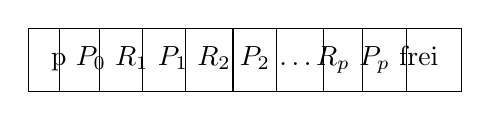
\begin{tikzpicture}

				\node at (2.35, 2.4) {p  $P_{0}$  $R_{1}$  $P_{1}$  $R_{2}$  $P_{2}$  \dots  $R_{p}$  $P_{p}$  frei};

				%Male ausgefülltes Rechteck
				%\fill[fill=lightgray](2.75, 2) rectangle+(0.4, 0.8);

				%Rechteck
				%     links hoehe         rechts hoehe
				\draw (-0.4,2) rectangle +(5.5, 0.8);

				%Senkrechte Striche
				\draw (0, 2) -- (0, 2.8)
							(0.5, 2) -- (0.5, 2.8)
							(1.05, 2) -- (1.05, 2.8)
							(1.6, 2) -- (1.6, 2.8)
							(2.2, 2) -- (2.2, 2.8)
							(2.75, 2) -- (2.75, 2.8)
							(3.35, 2) -- (3.35, 2.8)
							(3.85, 2) -- (3.85, 2.8)
							(4.4, 2) -- (4.4, 2.8)
							;

		\end{tikzpicture}
		\end{center}



	Wobei $P_{i}$ ein Zeiger auf einen weiteren inneren oder Blattknoten und $R_{i}$ ein Referenzschlüssel ist. p ist die Anzahl der Einträge. Es gilt: $k \leq p \leq 2 k$

	Blattknoten:

		\begin{center}
		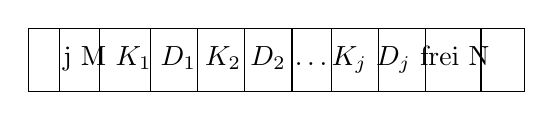
\begin{tikzpicture}

				\node at (2.35, 2.4) {j  M  $K_{1}$  $D_{1}$  $K_{2}$  $D_{2}$  \dots  $K_{j}$  $D_{j}$  frei   N};

				%Rechteck
				%     links hoehe         rechts hoehe
				\draw (-0.8,2) rectangle +(6.3, 0.8);

				%Senkrechte Striche
				\draw (-0.4, 2) -- (-0.4, 2.8)
							(0.1, 2) -- (0.1, 2.8)
							(0.75, 2) -- (0.75, 2.8)
							(1.35, 2) -- (1.35, 2.8)
							(1.95, 2) -- (1.95, 2.8)
							(2.55, 2) -- (2.55, 2.8)
							(3.05, 2) -- (3.05, 2.8)
							(3.65, 2) -- (3.65, 2.8)
							(4.25, 2) -- (4.25, 2.8)
							(4.95, 2) -- (4.95, 2.8)
							;

		\end{tikzpicture}
		\end{center}
	Wobei $K_{i}$ ein Referenzschlüssel ist und $D_{i}$ die Nutzdaten zum Schlüssel $K_{i}$. j ist die Anzahl der Einträge. Es gilt: $k^* \leq j \leq 2 k^*$. $M$ ist der Zeiger auf den vorherigen und $N$ der Zeiger auf den nächsten Blattknoten.

	\end{solution}

	\item Ist in einem B*-Baum jeder Schlüsselwert, der in einem inneren Knoten gespeichert ist, auch in einem Blattknoten vorhanden?

	\begin{solution}
		Nein. Es kann zum Beispiel durch Löschen eines Eintrags in einem Blattknoten die Situation entstehen,
		dass in einem inneren Knoten ein Referenzschlüssel vorkommt, der in keinem Blattknoten mehr enthalten ist. \\
		Selbstverständlich bleibt jedoch die Semantik erhalten, dass vor einem Referenzschlüssel nur Einträge mit niedrigeren
		oder gleichen Schlüsselwerten und nach dem Referenzschlüssel nur Einträge mit höheren Schlüsselwerten vorkommen.
	\end{solution}

	\item Welche Möglichkeiten fallen Ihnen ein, um Einträge wieder aus einem Index zu entfernen?

	\begin{solution}
		Die Einträge können direkt aus dem Index gelöscht werden. Das erfordert jedoch je nach Index und verwendeter Implementierung eine z.\,T. sehr aufwendige Reorganisation. Löschen in Hashtabellen mit quadratischem Sondieren ist komplex bis unmöglich, ohne kompletten Neuaufbau des Indexes. Löschen aus einem B-Baum kann eine ganze Reihe von Unterläufen und im Laufe der Unterlaufbehandlung wieder Überläufen erzeugen.

		Eine andere Möglichkeit ist, die Einträge als "`gelöscht"' zu markieren, ohne sie tatsächlich zu entfernen. So macht es z.\,B. auch Oracle in seinen B-Baum-Indizes. Hierdurch geht das Löschen sehr schnell. Der Speicherbedarf ist durch die gelöschten Elemente aber höher und kann je nach Struktur auch die Kosten für Einfügen und Suchen erhöhen. Der zusätzliche Aufwand hierfür ist abhängig von der Indeximplementierung und der Zahl der Löschvorgänge.

		Als Kompromisslösung bietet es sich an, Einträge als gelöscht zu markieren und ab einem gewissen Punkt, zum Beispiel einem bestimmten Prozentsatz von Platzhaltern in Bezug zur Gesamtzahl an Einträgen, die Tabelle neu aufzubauen. Bei Oracle stehen Informationen über den Zustand des Indexes bereit und der Administrator entscheidet darüber, wann ein Index neu aufgebaut werden soll.
	\end{solution}

	\item Welche Daten müssen und welche können in einem Index gespeichert werden?

	\begin{solution}
		Der Indexwert (Schlüssel) muss immer gespeichert werden. Was zusätzlich noch gespeichert wird, hängt davon ab, für was der Index benutzt werden soll:

		\begin{description}
			\item[Keine weiteren Informationen] Bereits nichts weiter als nur den Indexwert zu speichern kann Anfragen unterstützen, wenn oft überprüft werden soll, ob ein Schlüsselwert vorhanden ist, aber der zugehörige Satz nicht weiter interessiert (z.\,B. für Unique-Attribute oder zur Unterstützung einer \texttt{contains}-Funktion).
			\item[TID] Zusätzlich wird die Satzadresse des Satzes gespeichert. Dadurch wird der Schlüsselzugriff auf den Satz ermöglicht.
			\item[(TID +) Teil eines Satzes] Zusätzlich zum Schlüsselwert und der Satzadresse werden noch ein oder mehrere Felder gespeichert. Das erfordert natürlich einen höheren Platzbedarf, kann aber sinnvoll sein, wenn häufig Anfragen
			gestellt werden, die den Schlüssel und bestimmte Felder benutzen. Man spart sich den Zugriff über die Satzadresse, wenn die benötigten Felder bereits im Index stehen.
			Durch das Weglassen der TID erhält man eine Datenstruktur, die nur bei Anfragen auf die in der Struktur abgelegten Teile verwendet werden kann. Andernfalls ist der Index für diese Anfrage nicht benutzbar.
			\item[Ganzer Satz] Der ganze Satz wird im Index gespeichert. (Primärorganisation)
			\item[Mehrere TIDs, Teile von Sätzen, Sätze] Bei einem Index über ein nicht-eindeutiges Attribut kann es zu einem Schlüsselwert mehrere Tupel geben. Diese werden dann alle zusätzlich zum Schlüsselwert abgelegt. Hierfür sind, genauso wie für die Ablage variabel langer Sätze in einem Index, angepasste Index-Algorithmen notwendig, die variabel lange Einträge unterstützen.
			\item[TIDs, Teile von Sätzen, Sätze anderer Relationen] Bei einem Index über einen Primärschlüssel können sowohl die TIDs der beinhaltenden Relation als auch die TID der referenzierenden Relation mit Fremdschlüssel gespeichert werden, um den Join zu erleichtern. Natürlich lassen sich bei dieser Vorgehensweise alle anderen Optionen (Teile des Satzes, Ganzer Satz) genauso anwenden.
		\end{description}

		%Indexwert muss, TID, ganzes Tupel, Teil eines Tupels kann. Nur Indexwert könnte auch sinnvoll sein, wenn nur auf Vorhandensein geprüft werden soll.
	\end{solution}
\end{enumerate}

\begin{note}
Darauf hinweisen, dass B-Bäume der Standard bei der Implementierung von Indizes sind.

Außerdem darauf hinweisen, dass die Bezeichnung B$^\text{+}$-Baum dasselbe Konzept
meint, das wir als B*-Baum bezeichnen.
\end{note}




\beamertxt{\pagebreak}
\section{Eigenschaften von B-Bäumen}
Begründen Sie, warum der folgende Baum kein B-Baum ist.

\begin{center}
\begin{tikzpicture}
	%arrows
	\draw[thick, ->, >=stealth'] (1.85, 2) -- (0.6,0.8);
	\draw[thick, ->, >=stealth'] (3.25, 2) -- (5.5,0.8);
	%1st lvl
	\node at (2.35, 2.4) {4};

	\fill[fill=lightgray]
		(2.75, 2) rectangle+(0.4, 0.8);

	\draw (1.75,2) rectangle +(1.6, 0.8);

	\draw (1.95, 2) -- (1.95, 2.8)
 		(2.75, 2) -- (2.75, 2.8)
		(3.15, 2) -- (3.15, 2.8);
	%2nd lvl
	\node at (0.6, 0.4) {3};
	\node at (4.1, 0.4) {6};
	\node at (5.5, 0.4) {8};
	\node at (6.9, 0.4) {9};

	\fill[fill=lightgray]
		(1, 0) rectangle+(0.4, 0.8)
		(4.5, 0) rectangle+(0.4, 0.8)
		(5.9, 0) rectangle+(0.4, 0.8)
		(7.3, 0) rectangle+(0.4, 0.8);

	\draw (0,0) rectangle +(1.6,0.8)
		(3.5,0) rectangle +(4.4, 0.8);

	\draw (0.2, 0) -- (0.2, 0.8)
 		(1, 0) -- (1, 0.8)
		(1.4, 0) -- (1.4, 0.8)
 		(3.7, 0) -- (3.7, 0.8)
 		(4.5, 0) -- (4.5, 0.8)
		(4.9, 0) -- (4.9, 0.8)
		 (5.1, 0) -- (5.1, 0.8)
		 (5.9, 0) -- (5.9, 0.8)
		(6.3, 0) -- (6.3, 0.8)
		(6.5, 0) -- (6.5, 0.8)
		(7.3, 0) -- (7.3, 0.8)
		(7.7, 0) -- (7.7, 0.8);
\end{tikzpicture}
\end{center}

\begin{solution}
Es gilt: Jeder Knoten muss mindestens $k$ und darf höchstens $2k$ Einträge haben (außer dem Wurzelknoten). Für $k=1$ ist der linke Blattknoten konform, aber der rechte nicht. Für $k=2$ hingegen ist der rechte Blattknoten zulässig, aber der linke nicht. Daraus folgt, dass der angegebene Baum kein B-Baum ist.
\end{solution}




\section{Einfügen und Löschen im B-Baum}

\begin{enumerate}[a)]
	\item Fügen Sie in einen anfangs leeren B-Baum mit $k=2$ die Zahlen eins bis zwanzig in aufsteigender Reihenfolge ein. Was fällt Ihnen dabei auf?

\begin{solution}
Die Zahlen 1 bis 4 lassen sich problemlos in den Wurzelknoten einfügen.
\begin{center}
    \begin{tikzpicture}[
            start chain=0 going right,
            defaultNode/.style={defaultNode1},
        ]

        %Level0
		\draw pic {firstInnerNode={1}{2}{3}{4}{0}{0}{2}};
    \end{tikzpicture}
\end{center}

Bei 5 kommt es zum Wurzelsplitt und der Baum wächst um eins. Danach steht 3 in der Wurzel, 1 und 2 im linken Blattknoten und 4 und 5 im rechten Blattknoten.

\begin{center}
    \begin{tikzpicture}[
            start chain=0 going right,
            defaultNode/.style={defaultNode1},
        ]

        %Level0
		\draw pic {firstInnerNode={3}{}{}{}{0}{0}{5}};

        %Level1
        \draw pic {firstInnerNode={1}{2}{}{}{1}{1}{2}};
        \draw pic {innerNode={4}{5}{}{}{1}{2}};

        %Verbindungspfeile 0 - 1
        \draw pic {connect={0}{0}{1}};
        \draw pic {connect={0}{1}{2}};
    \end{tikzpicture}
\end{center}

6 und 7 können wieder ohne Splitt in den rechten Blattknoten eingefügt werden.

\begin{center}
    \begin{tikzpicture}[
            start chain=0 going right,
            defaultNode/.style={defaultNode1},
        ]

        %Level0
        \draw pic {firstInnerNode={3}{}{}{}{0}{0}{5}};

        %Level1
        \draw pic {firstInnerNode={1}{2}{}{}{1}{1}{2}};
        \draw pic {innerNode={4}{5}{6}{7}{1}{2}};

        %Verbindungspfeile 0 - 1
        \draw pic {connect={0}{0}{1}};
        \draw pic {connect={0}{1}{2}};
    \end{tikzpicture}
\end{center}

Das Einfügen der 8 führt zum Überlauf im rechten Blattknoten.
Der Knoten wird also an der 6 gesplittet, die in den Wurzelknoten wandert:

\begin{center}
    \begin{tikzpicture}[
            start chain=0 going right,
            defaultNode/.style={defaultNode1},
        ]

        %Level0
        \draw pic {firstInnerNode={3}{6}{}{}{0}{0}{8}};

        %Level1
        \draw pic {firstInnerNode={1}{2}{}{}{1}{1}{2}};
        \draw pic {innerNode={4}{5}{}{}{1}{2}};
        \draw pic {innerNode={7}{8}{}{}{1}{3}};

        %Verbindungspfeile 0 - 1
        \draw pic {connect={0}{0}{1}};
        \draw pic {connect={0}{1}{2}};
        \draw pic {connect={0}{2}{3}};
    \end{tikzpicture}
\end{center}

9 und 10 können wieder ohne Splitt eingefügt werden.
Beim Einfügen der 11 wird der rechte Blattknoten wieder gesplittet,
9 wird in den Wurzelknoten gezogen.
Das gleiche gilt für das Einfügen von 12, 13 und 14, nun ist der Wurzelknoten voll:

\begin{center}
    \begin{tikzpicture}[
            start chain=0 going right,
            defaultNode/.style={defaultNode2},
        ]

        %Level0
        \draw pic {firstInnerNode={3}{6}{9}{12}{0}{0}{8}};

        %Level1
        \draw pic {firstInnerNode={1}{2}{}{}{1}{1}{2}};
        \draw pic {innerNodeNarrow={4}{5}{}{}{1}{2}};
        \draw pic {innerNodeNarrow={7}{8}{}{}{1}{3}};
        \draw pic {innerNodeNarrow={10}{11}{}{}{1}{4}};
        \draw pic {innerNodeNarrow={13}{14}{}{}{1}{5}};

        %Verbindungspfeile 0 - 1
        \draw pic {connect={0}{0}{1}};
        \draw pic {connect={0}{1}{2}};
        \draw pic {connect={0}{2}{3}};
        \draw pic {connect={0}{3}{4}};
        \draw pic {connect={0}{4}{5}};
    \end{tikzpicture}
\end{center}

15 und 16 können wieder einfach in den rechten Blattknoten eingefügt werden.
Das Einfügen der 17 führt zum Splitt im rechten Blattknoten.
Da der Wurzelknoten aber bereits voll ist, führt das auch zum Wurzelsplitt.
Der entstehende Baum sieht dann so aus:

\begin{center}
    \begin{tikzpicture}[
            start chain=0 going right,
            defaultNode/.style={defaultNode2},
        ]

        %Level0
        \draw pic {firstInnerNode={9}{}{}{}{0}{0}{5}};

        %Level1
        \draw pic {firstInnerNode={3}{6}{}{}{1}{1}{2}};
        \draw pic {innerNodeVar={12}{15}{}{}{1}{2}{4}};

        %Level2
        \draw pic {firstInnerNode={1}{2}{}{}{2}{3}{0}};
        \draw pic {innerNodeNarrow={7}{8}{}{}{2}{5}};
        \draw pic {innerNode={10}{11}{}{}{2}{6}};
        \draw pic {innerNodeNarrow={16}{17}{}{}{2}{8}};

        %Level2.5
        \draw pic {firstInnerNode={4}{5}{}{}{3}{4}{3}};
        \draw pic {innerNodeVar={13}{14}{}{}{2}{7}{5.2}};


        %Verbindungspfeile
        \draw pic {connect={0}{0}{1}};
        \draw pic {connect={0}{1}{2}};
        \draw pic {connect={1}{0}{3}};
        \draw pic {connect={1}{1}{4}};
        \draw pic {connect={1}{2}{5}};
        \draw pic {connect={2}{0}{6}};
        \draw pic {connect={2}{1}{7}};
        \draw pic {connect={2}{2}{8}};
    \end{tikzpicture}
\end{center}

18 und 19 lassen sich nun wieder einfach in den letzten Blattknoten einfügen,
bei der 20 kommt es erneut zu einem Überlauf und einem Splitt.

Am Ende erhält man folgenden B-Baum:

\begin{center}
    \begin{tikzpicture}[
            start chain=0 going right,
            defaultNode/.style={defaultNode2},
        ]

        %Level0
        \draw pic {firstInnerNode={9}{}{}{}{0}{0}{6}};

        %Level1
        \draw pic {firstInnerNode={3}{6}{}{}{1}{1}{2.5}};
        \draw pic {innerNodeVar={12}{15}{18}{}{1}{2}{4.5}};

        %Level2
        \draw pic {firstInnerNode={1}{2}{}{}{2}{3}{0.5}};
        \draw pic {innerNodeVar={7}{8}{}{}{2}{5}{0.4}};
        \draw pic {innerNodeVar={13}{14}{}{}{2}{7}{2.4}};
        \draw pic {innerNodeVar={19}{20}{}{}{2}{9}{0.8}};

        %Level2.5
        \draw pic {firstInnerNode={4}{5}{}{}{3}{4}{3.5}};
        \draw pic {innerNodeVar={10}{11}{}{}{3}{6}{0.6}};
        \draw pic {innerNodeVar={16}{17}{}{}{3}{8}{2.7}};


        %Verbindungspfeile
        \draw pic {connect={0}{0}{1}};
        \draw pic {connect={0}{1}{2}};
        \draw pic {connect={1}{0}{3}};
        \draw pic {connect={1}{1}{4}};
        \draw pic {connect={1}{2}{5}};
        \draw pic {connect={2}{0}{6}};
        \draw pic {connect={2}{1}{7}};
        \draw pic {connect={2}{2}{8}};
        \draw pic {connect={2}{3}{9}};
    \end{tikzpicture}
\end{center}

Es fällt auf, dass der B-Baum nahezu minimale Auslastung aufweist. Dies liegt am sequentiellen Einfügen einer aufsteigenden Zahlenfolge in den B-Baum: Nach dem Aufspalten eines Knotens werden in den Knoten, der die kleineren Datensätze enthält, keine weiteren Werte mehr eingefügt.

Es fällt außerdem auf, dass in der Wurzelebene und in den inneren Ebenen jeweils immer nur Vielfache einer bestimmten Zahl $x$ auftreten. Bei genauerem Betrachten findet man heraus, dass sich diese Zahl $x$ für jede Ebene $i$ folgendermaßen berechnen lässt:
\[x = (k + 1)^{h - i}, i \in \mathbb{N}_{>0},\; h: \mathrm{H"ohe\ des\ Baums}\]

Erläuterung:
\begin{enumerate}[\arabic{enumii}.]
\item Wir stellen fest, dass alle „linken Kindblöcke“ durch das Splitten in unserem Beispiel immer zwei (also $k$) Elemente pro Block beinhalten.
\item Der linke Unterbaum besitzt in der ersten Ebene als Wurzel einen Knoten, welcher in der Ebene unter unserer betrachteten Ebene liegt.
Somit beinhaltet dieser zwei Elemente und drei Nachfolgeknoten, es sei denn, es handelt sich um einen Blattknoten.
\item Jeder dieser drei Nachfolger in der zweiten Ebene beinhaltet wieder zwei Elemente und hat damit drei Nachfolger, wenn es sich nicht um einen Blattknoten handelt.
Damit befinden sich in der dritten Ebene $3^2 = 9$ Knoten.
\item Führt man nun die Reihe fort kommt man mit der Unterbaumhöhe u auf die folgende Formel für die Anzahl der Elemente des linken Unterbaums:
\[(1 + 3 +3^2 +3^3 \ldots + 3^{u-1}) \cdot 2\]
\item Durch $u:= h-i$ mit h als Gesamthöhe und i als Ebene des betrachteten Knotens ergibt sich folgende allgemeine Summe:
\[(1 + (k+1) + (k+1)^2 + (k+1)^3 + \ldots + (k+1)^{h-i-1}) \cdot k = \left(\sum_{j=0}^{h-i-1} (k+1)^j\right)\cdot k \]
\item Das "`linkeste Element"' in unserer betrachteten Ebene ist damit dann das nächstgrößere Element, was sich mithilfe der geometrischen Reihe ($\sum_{i=0}^{n-1}q^i = \frac{q^n - 1}{q - 1}$) folgendermaßen berechnen lässt:
\begin{align*}
Wert &:= \text{Elemente im Unterbaum} + 1\\
& = \left(\sum_{j=0}^{h-i-1} (k+1)^j\right)\cdot k +1 \stackrel{\text{Geometrische Reihe}}{=} \frac{(k+1)^{h-i}-1}{k + 1 - 1}\cdot k + 1\\
&= (k+1)^{h-i}- 1 +1 = (k+1)^{h-i}
\end{align*}
\item Zwischen diesem "`linkesten Element"' und dem nächsten Element der Ebene befindet sich nun wieder ein Unterbaum, welcher die selbe Höhe wie der erste Unterbaum besitzt.
Damit enthält dieser wieder $(k+1)^{h-i} - 1$ Elemente und somit lautet der Wert des Elements $2\cdot (k+1)^{h-i}$.
\item Somit befinden sich in einer Ebene nur Vielfache des "`linkesten Elements"'.
\end{enumerate}
\end{solution}

\item Löschen Sie nun den Eintrag 9 und zeichnen Sie den entstehenden Baum.

\begin{solution}
Da ein innerer Eintrag gelöscht wird, muss er durch den direkten Vorgänger oder Nachfolger ersetzt werden.
Da Vorgänger- und Nachfolgerblattknoten gleich viele Einträge haben, können wir uns frei zwischen Vorgänger und Nachfolger entscheiden. Wir nehmen hier den Vorgänger 8:

\begin{note}
	Wir nehmen die 8, weil die 10 einfacher ist, da im rechten Teilbaum die 18 exisitiert, und so kein Wurzel-merge n\"otig ist.
\end{note}

\begin{center}
    \begin{tikzpicture}[
            start chain=0 going right,
            defaultNode/.style={defaultNode2},
        ]

        %Level0
        \draw pic {firstInnerNode={8}{}{}{}{0}{0}{6}};

        %Level1
        \draw pic {firstInnerNode={3}{6}{}{}{1}{1}{2.5}};
        \draw pic {innerNodeVar={12}{15}{18}{}{1}{2}{4.5}};

        %Level2
        \draw pic {firstInnerNode={1}{2}{}{}{2}{3}{0.5}};
        \draw pic {innerNodeVar={7}{}{}{}{2}{5}{0.4}};
        \draw pic {innerNodeVar={13}{14}{}{}{2}{7}{2.6}};
        \draw pic {innerNodeVar={19}{20}{}{}{2}{9}{0.6}};

        %Level2.5
        \draw pic {firstInnerNode={4}{5}{}{}{3}{4}{3.5}};
        \draw pic {innerNodeVar={10}{11}{}{}{3}{6}{0.6}};
        \draw pic {innerNodeVar={16}{17}{}{}{3}{8}{2.7}};


        %Verbindungspfeile
        \draw pic {connect={0}{0}{1}};
        \draw pic {connect={0}{1}{2}};
        \draw pic {connect={1}{0}{3}};
        \draw pic {connect={1}{1}{4}};
        \draw pic {connect={1}{2}{5}};
        \draw pic {connect={2}{0}{6}};
        \draw pic {connect={2}{1}{7}};
        \draw pic {connect={2}{2}{8}};
        \draw pic {connect={2}{3}{9}};
    \end{tikzpicture}
\end{center}


Dadurch entsteht ein Unterlauf im Blattknoten,
der deshalb mit dem Elternknoten gemischt werden muss:

\begin{center}
    \begin{tikzpicture}[
            start chain=0 going right,
            defaultNode/.style={defaultNode2},
        ]

        %Level0
        \draw pic {firstInnerNode={8}{}{}{}{0}{0}{6}};

        %Level1
        \draw pic {firstInnerNode={3}{}{}{}{1}{1}{2.5}};
        \draw pic {innerNodeVar={12}{15}{18}{}{1}{2}{4.5}};

        %Level2
        \draw pic {firstInnerNode={1}{2}{}{}{2}{3}{0.5}};
        \draw pic {innerNodeVar={4}{5}{6}{7}{3}{4}{0.5}};
        \draw pic {innerNodeVar={13}{14}{}{}{2}{7}{1.7}};
        \draw pic {innerNodeVar={19}{20}{}{}{2}{9}{0.8}};

        %Level2.5
        \draw pic {firstInnerNode={10}{11}{}{}{3}{6}{6.6}};
        \draw pic {innerNodeVar={16}{17}{}{}{3}{8}{2.9}};


        %Verbindungspfeile
        \draw pic {connect={0}{0}{1}};
        \draw pic {connect={0}{1}{2}};
        \draw pic {connect={1}{0}{3}};
        \draw pic {connect={1}{1}{4}};
        \draw pic {connect={2}{0}{6}};
        \draw pic {connect={2}{1}{7}};
        \draw pic {connect={2}{2}{8}};
        \draw pic {connect={2}{3}{9}};
    \end{tikzpicture}
\end{center}

Nun besteht aber im linken inneren Knoten ein Unterlauf, der aufgelöst werden muss.
Dazu wird mit der Wurzel gemischt. Es entsteht ein Überlauf in der (neuen) Wurzel,
die deshalb gesplittet werden muss. Ergebnis:

\begin{center}
    \begin{tikzpicture}[
            start chain=0 going right,
            defaultNode/.style={defaultNode2},
        ]

        %Level0
        \draw pic {firstInnerNode={12}{}{}{}{0}{0}{6}};

        %Level1
        \draw pic {firstInnerNode={3}{8}{}{}{1}{1}{2.5}};
        \draw pic {innerNodeVar={15}{18}{}{}{1}{2}{4.5}};

        %Level2
        \draw pic {firstInnerNode={1}{2}{}{}{2}{3}{0}};
        \draw pic {innerNodeVar={10}{11}{}{}{2}{5}{0.4}};
        \draw pic {innerNodeVar={13}{14}{}{}{2}{7}{1}};
        \draw pic {innerNodeVar={19}{20}{}{}{2}{9}{0.8}};

        %Level2.5
        \draw pic {firstInnerNode={4}{5}{6}{7}{3}{4}{2.6}};
        \draw pic {innerNodeVar={16}{17}{}{}{3}{8}{4.9}};


        %Verbindungspfeile
        \draw pic {connect={0}{0}{1}};
        \draw pic {connect={0}{1}{2}};
        \draw pic {connect={1}{0}{3}};
        \draw pic {connect={1}{1}{4}};
        \draw pic {connect={1}{2}{5}};
        \draw pic {connect={2}{0}{7}};
        \draw pic {connect={2}{1}{8}};
        \draw pic {connect={2}{2}{9}};
    \end{tikzpicture}
\end{center}

\end{solution}

\end{enumerate}


\begin{deeper}
\section{B-Baum die Zweite}
Fügen Sie nun die folgenden 20 Zahlen in der vorgegebenen Reihenfolge in einen leeren B-Baum mit \( k=2 \) ein:\\
3, 14, 15, 92, 65, 35, 89, 79, 32, 38, 46, 26, 43, 50, 28, 84, 19, 71, 69, 39

\begin{note}
	Die Zahlen 3, 14, 15, 92 lassen sich problemlos in den Wurzelknoten einfügen.
	\begin{center}
		\begin{tikzpicture}[
		start chain=0 going right,
		defaultNode/.style={defaultNode1},
		]

		%Level0
		\draw pic {firstInnerNode={3}{14}{15}{92}{0}{0}{2}};
		\end{tikzpicture}
	\end{center}

Bei 65 kommt es zum Wurzelsplitt und der Baum wächst um eins.
Danach stehen 15 in der Wurzel, 3 und 14 im linken Blattknoten und 65 und 92 im rechten Blattknoten.

	\begin{center}
		\begin{tikzpicture}[
		start chain=0 going right,
		defaultNode/.style={defaultNode1},
		]

		%Level0
		\draw pic {firstInnerNode={15}{}{}{}{0}{0}{5}};

		%Level1
		\draw pic {firstInnerNode={3}{14}{}{}{1}{1}{2}};
		\draw pic {innerNode={65}{92}{}{}{1}{2}};

		%Verbindungspfeile 0 - 1
		\draw pic {connect={0}{0}{1}};
		\draw pic {connect={0}{1}{2}};
		\end{tikzpicture}
	\end{center}

35 und 89 können wieder ohne Splitt in den rechten Blattknoten eingefügt werden, bis es dann bei der 79 zu einem Splitt kommt.

	\begin{center}
		\begin{tikzpicture}[
		start chain=0 going right,
		defaultNode/.style={defaultNode1},
		]

		%Level0
		\draw pic {firstInnerNode={15}{79}{}{}{0}{0}{5}};

		%Level1
		\draw pic {firstInnerNode={3}{14}{}{}{1}{1}{2}};
		\draw pic {innerNode={35}{65}{}{}{1}{2}};
		\draw pic {innerNode={89}{92}{}{}{1}{3}};

		%Verbindungspfeile 0 - 11
		\draw pic {connect={0}{0}{1}};
		\draw pic {connect={0}{1}{2}};
		\draw pic {connect={0}{2}{3}};
		\end{tikzpicture}
	\end{center}

32 und 38 können wieder ohne Probleme in den mittleren Blattknoten eingefügt werden. Erst bei der 46 kommt es wieder zu einem Überlauf.

	\begin{center}
		\begin{tikzpicture}[
		start chain=0 going right,
		defaultNode/.style={defaultNode1},
		]

		%Level0
		\draw pic {firstInnerNode={15}{38}{79}{}{0}{0}{8}};

		%Level1
		\draw pic {firstInnerNode={3}{14}{}{}{1}{1}{2}};
		\draw pic {innerNode={32}{35}{}{}{1}{2}};
		\draw pic {innerNode={46}{65}{}{}{1}{3}};
		\draw pic {innerNode={89}{92}{}{}{1}{4}};

		%Verbindungspfeile 0 - 1
		\draw pic {connect={0}{0}{1}};
		\draw pic {connect={0}{1}{2}};
		\draw pic {connect={0}{2}{3}};
		\draw pic {connect={0}{3}{4}};
		\end{tikzpicture}
	\end{center}

	26, 43, 50, 28 und 84 können wieder ohne Splitt eingefügt werden.
	Beim Einfügen der 19 wird der zweite Blattknoten gesplittet,
	28 wird in den Wurzelknoten gezogen.

	\begin{center}
		\begin{tikzpicture}[
		start chain=0 going right,
		defaultNode/.style={defaultNode2},
		]

		%Level0
		\draw pic {firstInnerNode={15}{28}{38}{79}{0}{0}{8}};

		%Level1
		\draw pic {firstInnerNode={3}{14}{}{}{1}{1}{2}};
		\draw pic {innerNodeNarrow={19}{26}{}{}{1}{2}};
		\draw pic {innerNodeNarrow={32}{35}{}{}{1}{3}};
		\draw pic {innerNodeNarrow={43}{46}{50}{65}{1}{4}};
		\draw pic {innerNodeNarrow={84}{89}{92}{}{1}{5}};

		%Verbindungspfeile 0 - 1
		\draw pic {connect={0}{0}{1}};
		\draw pic {connect={0}{1}{2}};
		\draw pic {connect={0}{2}{3}};
		\draw pic {connect={0}{3}{4}};
		\draw pic {connect={0}{4}{5}};
		\end{tikzpicture}
	\end{center}

Das Einfügen der 71 führt zum Splitt im Blattknoten. die 50 wird nach oben geschoben und es kommt zum Überlauf im Wurzelknoten. Dieser wird gesplittet und die 38 wandert nach oben.
Der entstehende Baum sieht dann so aus:

	\begin{center}
		\begin{tikzpicture}[
		start chain=0 going right,
		defaultNode/.style={defaultNode2},
		]

		%Level0
		\draw pic {firstInnerNode={38}{}{}{}{0}{0}{8}};

		%Level1
		\draw pic {firstInnerNode={15}{28}{}{}{1}{1}{4}};
		\draw pic {innerNodeVar={50}{79}{}{}{1}{2}{4}};

		%Level2
		\draw pic {firstInnerNode={3}{14}{}{}{2}{3}{1}};
		\draw pic {innerNodeVar={32}{35}{}{}{2}{5}{0.8}};
		\draw pic {innerNodeNarrow={43}{46}{}{}{2}{6}};
		\draw pic {innerNodeVar={84}{89}{92}{}{2}{8}{0.8}};

		%Level2.5
		\draw pic {firstInnerNode={19}{26}{}{}{2.5}{4}{4}};
		\draw pic {innerNodeVar={65}{71}{}{}{2.5}{7}{4}};

		%Verbindungspfeile
		\draw pic {connect={0}{0}{1}};
		\draw pic {connect={0}{1}{2}};
		\draw pic {connect={1}{0}{3}};
		\draw pic {connect={1}{1}{4}};
		\draw pic {connect={1}{2}{5}};
		\draw pic {connect={2}{0}{6}};
		\draw pic {connect={2}{1}{7}};
		\draw pic {connect={2}{2}{8}};
		\end{tikzpicture}
	\end{center}

Final werden nun die 69 und 39 eingefügt.

Am Ende erhält man folgenden B-Baum:

	\begin{center}
	\begin{tikzpicture}[
	start chain=0 going right,
	defaultNode/.style={defaultNode2},
	]

	%Level0
	\draw pic {firstInnerNode={38}{}{}{}{0}{0}{8}};

	%Level1
	\draw pic {firstInnerNode={15}{28}{}{}{1}{1}{4}};
	\draw pic {innerNodeVar={50}{79}{}{}{1}{2}{4}};

	%Level2
	\draw pic {firstInnerNode={3}{14}{}{}{2}{3}{1}};
	\draw pic {innerNodeVar={32}{35}{}{}{2}{5}{0.8}};
	\draw pic {innerNodeNarrow={39}{43}{46}{}{2}{6}};
	\draw pic {innerNodeVar={84}{89}{92}{}{2}{8}{0.8}};

	%Level2.5
	\draw pic {firstInnerNode={19}{26}{}{}{2.5}{4}{4}};
	\draw pic {innerNodeVar={65}{69}{71}{}{2.5}{7}{4}};

	%Verbindungspfeile
	\draw pic {connect={0}{0}{1}};
	\draw pic {connect={0}{1}{2}};
	\draw pic {connect={1}{0}{3}};
	\draw pic {connect={1}{1}{4}};
	\draw pic {connect={1}{2}{5}};
	\draw pic {connect={2}{0}{6}};
	\draw pic {connect={2}{1}{7}};
	\draw pic {connect={2}{2}{8}};
	\end{tikzpicture}
\end{center}
\end{note}

\end{deeper}

\section{B*-Baum}
\label{B*}

Gegeben ist ein anfangs leerer B*-Baum. Die maximale Zahl der Einträge für einen inneren Knoten beträgt $2k$, $k = 2$. Die maximale Zahl der Einträge in einem Blattknoten beträgt $2k^*$, $k^* = 1$. Es sollen Tupel bestehend aus dem Schlüssel (einer Ganzzahl) und einem String der Länge $3$ gespeichert werden. Führen Sie die im Folgenden angegebenen Einfüge- und Löschoperationen im B*-Baum durch. Wenn sich dessen Struktur dabei ändert, zeichnen Sie den B*-Baum neu!

\begin{enumerate}[a)]
  \item Fügen Sie die folgenden Tupel in der angegeben Reihenfolge in den B*-Baum ein: \textit{(1,fan), (13,gct), (7,xxe), (8,lwc), (22,vkw), (5,wym), (2,gzw), (10,ycc)}

	\begin{solution}
Für ViseAUD: 1 fan, 13 gct, 7 xxe, 8 lwc, 22 vkw, 5 wym, 2 gzw, 10 ycc

Einfügen der Tupel mit Schlüssel 1 und 13. Der Wurzelknoten ist initial noch ein Blattknoten.

	\begin{center}
		\begin{tikzpicture}[
				start chain=0 going right,
				defaultNode/.style={defaultNode1},
			]

			%Level0
			\draw pic {firstLeafNode={1}{(fan)}{13}{(gct)}{0}{0}{0}};

		\end{tikzpicture}
  \end{center}

Durch Einfügen des Tupels mit Schlüssel 7 entsteht ein Überlauf im Wurzelknoten.
Es kommt zum Splitt im Wurzelknoten.
Dadurch ist der Wurzelknoten jetzt ein innerer Knoten und es existieren zwei Blattknoten.
Der Baum wächst um eins.

	\begin{center}
		\begin{tikzpicture}[
				start chain=0 going right,
				start chain=1 going right,
				defaultNode/.style={defaultNode1},
			]

			%Level0
			\draw pic {firstInnerNode={7}{}{}{}{0}{0}{2}};

            %Level1
            \draw pic {firstLeafNode={1}{(fan)}{7}{(xxe)}{1}{1}{0}};
            \draw pic {leafNode={13}{(gct)}{}{}{1}{2}};

            %Verbindungspfeile 0 - 1
            \draw pic {connect={0}{0}{1}};
            \draw pic {connect={0}{1}{2}};

		\end{tikzpicture}
    \end{center}

Einfügen des Tupels mit Schlüssel 8.

	\begin{center}
		\begin{tikzpicture}[
				start chain=0 going right,
				start chain=1 going right,
				defaultNode/.style={defaultNode1},
			]

			%Level0
			\draw pic {firstInnerNode={7}{}{}{}{0}{0}{2}};

            %Level1
            \draw pic {firstLeafNode={1}{(fan)}{7}{(xxe)}{1}{1}{0}};
            \draw pic {leafNode={8}{(lwc)}{13}{(gct)}{1}{2}};

            %Verbindungspfeile 0 - 1
            \draw pic {connect={0}{0}{1}};
            \draw pic {connect={0}{1}{2}};

    \end{tikzpicture}
    \end{center}

Einfügen des Tupels mit Schlüssel 22. Im zweiten Blattknoten entsteht ein Überlauf. Es werden ein neuer Blattknoten erzeugt und im Wurzelknoten ein neuer Eintrag hinzugefügt.

	\begin{center}
		\begin{tikzpicture}[
				start chain=0 going right,
				start chain=1 going right,
				defaultNode/.style={defaultNode1},
			]

			%Level0
			\draw pic {firstInnerNode={7}{13}{}{}{0}{0}{3}};

            %Level1
            \draw pic {firstLeafNode={1}{(fan)}{7}{(xxe)}{1}{1}{0}};
            \draw pic {leafNode={8}{(lwc)}{13}{(gct)}{1}{2}};
            \draw pic {leafNode={22}{(vkw)}{}{}{1}{3}};

            %Verbindungspfeile 0 - 1
            \draw pic {connect={0}{0}{1}};
            \draw pic {connect={0}{1}{2}};
            \draw pic {connect={0}{2}{3}};

		\end{tikzpicture}
    \end{center}

Einfügen des Tupels mit Schlüssel 5. Im ersten Blattknoten entsteht ein Überlauf. Es werden ein neuer Blattknoten erzeugt und im Wurzelknoten ein neuer Eintrag hinzugefügt.

	\begin{center}
		\begin{tikzpicture}[
				start chain=0 going right,
				start chain=1 going right,
				defaultNode/.style={defaultNode1},
			]

			%Level0
			\draw pic {firstInnerNode={5}{7}{13}{}{0}{0}{4}};

            %Level1
            \draw pic {firstLeafNode={1}{(fan)}{5}{(wym)}{1}{1}{0}};
            \draw pic {leafNode={7}{(xxe)}{}{}{1}{2}};
            \draw pic {leafNode={8}{(lwc)}{13}{(gct)}{1}{3}};
            \draw pic {leafNode={22}{(vkw)}{}{}{1}{4}};

            %Verbindungspfeile 0 - 1
            \draw pic {connect={0}{0}{1}};
            \draw pic {connect={0}{1}{2}};
            \draw pic {connect={0}{2}{3}};
            \draw pic {connect={0}{3}{4}};

		\end{tikzpicture}
    \end{center}

Einfügen des Tupels mit Schlüssel 2. Im ersten Blattknoten entsteht ein Überlauf. Es werden ein neuer Blattknoten erzeugt und im Wurzelknoten ein neuer Eintrag hinzugefügt.

	\begin{center}
		\begin{tikzpicture}[
				start chain=0 going right,
				start chain=1 going right,
				defaultNode/.style={defaultNode1},
			]

			%Level0
			\draw pic {firstInnerNode={2}{5}{7}{13}{0}{0}{5}};

            %Level1
            \draw pic {firstLeafNode={1}{(fan)}{2}{(gzw)}{1}{1}{0}};
            \draw pic {leafNode={5}{(wym)}{}{}{1}{2}};
            \draw pic {leafNode={7}{(xxe)}{}{}{1}{3}};
            \draw pic {leafNode={8}{(lwc)}{13}{(gct)}{1}{4}};
            \draw pic {leafNode={22}{(vkw)}{}{}{1}{5}};

            %Verbindungspfeile 0 - 1
            \draw pic {connect={0}{0}{1}};
            \draw pic {connect={0}{1}{2}};
            \draw pic {connect={0}{2}{3}};
            \draw pic {connect={0}{3}{4}};
            \draw pic {connect={0}{4}{5}};

		\end{tikzpicture}
    \end{center}

Einfügen des Tupels mit Schlüssel 10. Im vierten Blattknoten entsteht ein Überlauf. Es werden ein neuer Blattknoten erzeugt und im Wurzelknoten ein neuer Eintrag hinzugefügt. Es kommt zum Überlauf im Wurzelknoten. Es werden zwei neue innere Knoten erzeugt mit jeweils zwei Einträgen. Der Wurzelknoten hat einen Eintrag.

	\begin{center}
        \scalebox{0.9}{%
		\begin{tikzpicture}[
				start chain=0 going right,
				start chain=1 going right,
				start chain=2 going right,
				defaultNode/.style={defaultNode1}
			]

			%Level0
			\draw pic {firstInnerNode={7}{}{}{}{0}{0}{6}};

			%Level1
			\draw pic {firstInnerNode={2}{5}{}{}{1}{1}{4}};
			\draw pic {innerNode={10}{13}{}{}{1}{2}};

			%Level2
			\draw pic {firstLeafNode={1}{(fan)}{2}{(gzw)}{2}{3}{0}};
			\draw pic {leafNode={5}{(wym)}{}{}{2}{4}};
			\draw pic {leafNode={7}{(xxe)}{}{}{2}{5}};
			\draw pic {leafNode={8}{(lwc)}{10}{(ycc)}{2}{6}};
			\draw pic {leafNode={13}{(gct)}{}{}{2}{7}};
			\draw pic {leafNode={22}{(vkw)}{}{}{2}{8}};

			%Verbindungspfeile
			%Level 0 -> 1
			\draw pic {connect={0}{0}{1}};
			\draw pic {connect={0}{1}{2}};
			%Level 1->2
			\draw pic {connect={1}{0}{3}};
			\draw pic {connect={1}{1}{4}};
			\draw pic {connect={1}{2}{5}};
			\draw pic {connect={2}{0}{6}};
			\draw pic {connect={2}{1}{7}};
			\draw pic {connect={2}{2}{8}};

		\end{tikzpicture}
        }
    \end{center}
	\end{solution}

	\item Löschen Sie jetzt den Datensatz mit Schlüssel $10$, danach den mit Schlüssel $13$.

	\begin{solution}
	Löschen des Tupels mit Schlüssel 10 (also $(10,ycc)$) aus dem vierten Blattknoten.\\

	\begin{center}
		\begin{tikzpicture}[
				start chain=0 going right,
				start chain=1 going right,
				start chain=2 going right,
				defaultNode/.style={defaultNode1},
			]

			%Level0
			\draw pic {firstInnerNode={7}{}{}{}{0}{0}{6}};

			%Level1
			\draw pic {firstInnerNode={2}{5}{}{}{1}{1}{4}};
			\draw pic {innerNode={10}{13}{}{}{1}{2}};

			%Level2
			\draw pic {firstLeafNode={1}{(fan)}{2}{(gzw)}{2}{3}{0}};
			\draw pic {leafNode={5}{(wym)}{}{}{2}{4}};
			\draw pic {leafNode={7}{(xxe)}{}{}{2}{5}};
			\draw pic {leafNode={8}{(lwc)}{}{}{2}{6}};
			\draw pic {leafNode={13}{(gct)}{}{}{2}{7}};
			\draw pic {leafNode={22}{(vkw)}{}{}{2}{8}};

			%Verbindungspfeile
			%Level 0 -> 1
			\draw pic {connect={0}{0}{1}};
			\draw pic {connect={0}{1}{2}};
			%Level 1->2
			\draw pic {connect={1}{0}{3}};
			\draw pic {connect={1}{1}{4}};
			\draw pic {connect={1}{2}{5}};
			\draw pic {connect={2}{0}{6}};
			\draw pic {connect={2}{1}{7}};
			\draw pic {connect={2}{2}{8}};

		\end{tikzpicture}
    \end{center}

	Löschen von 13 führt zu Unterlauf in Blattknoten.

	\begin{center}
		\begin{tikzpicture}[
				start chain=0 going right,
				start chain=1 going right,
				start chain=2 going right,
				defaultNode/.style={defaultNode1},
			]

			%Level0
			\draw pic {firstInnerNode={7}{}{}{}{0}{0}{5}};

			%Level1
			\draw pic {firstInnerNode={2}{5}{}{}{1}{1}{3}};
			\draw pic {innerNode={10}{13}{}{}{1}{2}};

			%Level2
			\draw pic {firstLeafNode={1}{(fan)}{2}{(gzw)}{2}{3}{0}};
			\draw pic {leafNode={5}{(wym)}{}{}{2}{4}};
			\draw pic {leafNode={7}{(xxe)}{}{}{2}{5}};
			\draw pic {leafNode={8}{(lwc)}{}{}{2}{6}};
			\draw pic {leafNode={}{}{}{}{2}{7}};
			\draw pic {leafNode={22}{(vkw)}{}{}{2}{8}};

			%Verbindungspfeile
			%Level 0 -> 1
			\draw pic {connect={0}{0}{1}};
			\draw pic {connect={0}{1}{2}};
			%Level 1->2
			\draw pic {connect={1}{0}{3}};
			\draw pic {connect={1}{1}{4}};
			\draw pic {connect={1}{2}{5}};
			\draw pic {connect={2}{0}{6}};
			\draw pic {connect={2}{1}{7}};
			\draw pic {connect={2}{2}{8}};


		\end{tikzpicture}
    \end{center}

Untergelaufenen Blattknoten mit benachbartem Knoten mischen (hier mit rechtem Nachbarknoten). Entfernen des entsprechenden Eintrags im inneren Knoten. Führt zu Unterlauf im inneren Knoten.

	\begin{center}
		\begin{tikzpicture}[
				start chain=0 going right,
				start chain=1 going right,
				start chain=2 going right,
				defaultNode/.style={defaultNode1},
			]

			%Level0
			\draw pic {firstInnerNode={7}{}{}{}{0}{0}{5}};

			%Level1
			\draw pic {firstInnerNode={2}{5}{}{}{1}{1}{3}};
			\draw pic {innerNode={10}{}{}{}{1}{2}};

			%Level2
			\draw pic {firstLeafNode={1}{(fan)}{2}{(gzw)}{2}{3}{0}};
			\draw pic {leafNode={5}{(wym)}{}{}{2}{4}};
			\draw pic {leafNode={7}{(xxe)}{}{}{2}{5}};
			\draw pic {leafNode={8}{(lwc)}{}{}{2}{6}};
			\draw pic {leafNode={22}{(vkw)}{}{}{2}{7}};

			%Verbindungspfeile
			%Level 0 -> 1
			\draw pic {connect={0}{0}{1}};
			\draw pic {connect={0}{1}{2}};
			%Level 1->2
			\draw pic {connect={1}{0}{3}};
			\draw pic {connect={1}{1}{4}};
			\draw pic {connect={1}{2}{5}};
			\draw pic {connect={2}{0}{6}};
			\draw pic {connect={2}{1}{7}};

		\end{tikzpicture}
    \end{center}

Beide inneren Knoten mischen. Führt zu Unterlauf im Wurzelknoten. Baum schrumpft um eins.

	\begin{center}
		\begin{tikzpicture}[
				start chain=0 going right,
				start chain=1 going right,
				defaultNode/.style={defaultNode1},
			]

			%Level0
			\draw pic {firstInnerNode={2}{5}{7}{10}{0}{0}{5}};

            %Level1
            \draw pic {firstLeafNode={1}{(fan)}{2}{(gzw)}{1}{1}{0}};
            \draw pic {leafNode={5}{(wym)}{}{}{1}{2}};
            \draw pic {leafNode={7}{(xxe)}{}{}{1}{3}};
            \draw pic {leafNode={8}{(lwc)}{}{}{1}{4}};
            \draw pic {leafNode={22}{(vkw)}{}{}{1}{5}};

            %Verbindungspfeile 0 - 1
            \draw pic {connect={0}{0}{1}};
            \draw pic {connect={0}{1}{2}};
            \draw pic {connect={0}{2}{3}};
            \draw pic {connect={0}{3}{4}};
            \draw pic {connect={0}{4}{5}};

		\end{tikzpicture}
    \end{center}

	\end{solution}

\end{enumerate}



\begin{deeper}
\section{B*-Baum die Zweite}

Es gelten die selben Voraussetzungen wie in \ref{B*}.

\begin{enumerate}[a)]
	\item Fügen Sie die folgenden Tupel in der angegebenen Reihenfolge in den B*-Baum ein:\\
\textit{(2,wel), (71,swo), (82,st?), (13,aha), (81,hli), (8,che), (28,zah), (42,ble), (45,lda), (22,nei)
}
\begin{note}
	Einfügen der Tupel mit Schlüssel 2 und 71. Der Wurzelknoten ist initial noch ein Blattknoten.

	\begin{center}
		\begin{tikzpicture}[
		start chain=0 going right,
		defaultNode/.style={defaultNode1},
		]

		%Level0
		\draw pic {firstLeafNode={2}{(wel)}{71}{(swo)}{0}{0}{0}};

		\end{tikzpicture}
	\end{center}

Durch Einfügen des Tupels mit Schlüssel 82 entsteht ein Überlauf im Wurzelknoten.
Es kommt zum Splitt im Wurzelknoten.
Dadurch ist der Wurzelknoten jetzt ein innerer Knoten und es existieren zwei Blattknoten.
Der Baum wächst um eins.

	\begin{center}
		\begin{tikzpicture}[
		start chain=0 going right,
		start chain=1 going right,
		defaultNode/.style={defaultNode1},
		]

		%Level0
		\draw pic {firstInnerNode={71}{}{}{}{0}{0}{2}};

		%Level1
		\draw pic {firstLeafNode={2}{(wel)}{71}{(swo)}{1}{1}{0}};
		\draw pic {leafNode={82}{(st?)}{}{}{1}{2}};

		%Verbindungspfeile 0 - 1
		\draw pic {connect={0}{0}{1}};
		\draw pic {connect={0}{1}{2}};

		\end{tikzpicture}
	\end{center}

Das Einfügen des Tupels mit Schlüssel 13 führt wieder zu einem Überlauf und Splitt im Blattknoten.

	\begin{center}
		\begin{tikzpicture}[
		start chain=0 going right,
		start chain=1 going right,
		defaultNode/.style={defaultNode1},
		]

		%Level0
		\draw pic {firstInnerNode={13}{71}{}{}{0}{0}{2}};

		%Level1
		\draw pic {firstLeafNode={2}{(wel)}{13}{(aha)}{1}{1}{0}};
		\draw pic {leafNode={71}{(swo)}{}{}{1}{2}};
		\draw pic {leafNode={82}{(st?)}{}{}{1}{3}};

		%Verbindungspfeile 0 - 1
		\draw pic {connect={0}{0}{1}};
		\draw pic {connect={0}{1}{2}};
		\draw pic {connect={0}{2}{3}};
		\end{tikzpicture}
	\end{center}

Einfügen des Tupels mit Schlüssel 81.

	\begin{center}
		\begin{tikzpicture}[
		start chain=0 going right,
		start chain=1 going right,
		defaultNode/.style={defaultNode1},
		]

		%Level0
		\draw pic {firstInnerNode={13}{71}{}{}{0}{0}{2}};

		%Level1
		\draw pic {firstLeafNode={2}{(wel)}{13}{(aha)}{1}{1}{0}};
		\draw pic {leafNode={71}{(swo)}{}{}{1}{2}};
		\draw pic {leafNode={81}{(hli)}{82}{(st?)}{1}{3}};

		%Verbindungspfeile 0 - 1
		\draw pic {connect={0}{0}{1}};
		\draw pic {connect={0}{1}{2}};
		\draw pic {connect={0}{2}{3}};

		\end{tikzpicture}
	\end{center}

Einfügen des Tupels mit Schlüssel 8. Im ersten Blattknoten entsteht ein Überlauf. Es werden ein neuer Blattknoten erzeugt und im Wurzelknoten ein neuer Eintrag hinzugefügt.

	\begin{center}
		\begin{tikzpicture}[
		start chain=0 going right,
		start chain=1 going right,
		defaultNode/.style={defaultNode1},
		]

		%Level0
		\draw pic {firstInnerNode={8}{13}{71}{}{0}{0}{3}};

		%Level1
		\draw pic {firstLeafNode={2}{(wel)}{8}{(che)}{1}{1}{0}};
		\draw pic {leafNode={13}{(aha)}{}{}{1}{2}};
		\draw pic {leafNode={71}{(swo)}{}{}{1}{3}};
		\draw pic {leafNode={81}{(hli)}{82}{(st?)}{1}{4}};

		%Verbindungspfeile 0 - 1
		\draw pic {connect={0}{0}{1}};
		\draw pic {connect={0}{1}{2}};
		\draw pic {connect={0}{2}{3}};
		\draw pic {connect={0}{3}{4}};

		\end{tikzpicture}
	\end{center}

Das Einfügen des Tupels mit Schlüssel 28 verläuft ohne Überläufe. Beim Einfügen der 42 kommt es aber wieder zu einem Überlauf. Es werden ein neuer Blattknoten erzeugt und im Wurzelknoten ein neuer Eintrag hinzugefügt.

Das Einfügen der 45 verläuft nun wieder ohne Probleme.

	\begin{center}
		\begin{tikzpicture}[
		start chain=0 going right,
		start chain=1 going right,
		defaultNode/.style={defaultNode1},
		]

		%Level0
		\draw pic {firstInnerNode={8}{13}{42}{71}{0}{0}{3}};

		%Level1
		\draw pic {firstLeafNode={2}{(wel)}{8}{(che)}{1}{1}{0}};
		\draw pic {leafNode={13}{(aha)}{}{}{1}{2}};
		\draw pic {leafNode={28}{(zah)}{42}{(ble)}{1}{3}};
		\draw pic {leafNode={45}{(lda)}{71}{(swo)}{1}{4}};
		\draw pic {leafNode={81}{(hli)}{82}{(st?)}{1}{5}};

		%Verbindungspfeile 0 - 1
		\draw pic {connect={0}{0}{1}};
		\draw pic {connect={0}{1}{2}};
		\draw pic {connect={0}{2}{3}};
		\draw pic {connect={0}{3}{4}};
		\draw pic {connect={0}{4}{5}};

		\end{tikzpicture}
	\end{center}

Das Einfügen der 22 erzeugt nun einen Überlauf im Blattknoten und darauf im Wurzelknoten.

	\begin{center}
		\begin{tikzpicture}[
		start chain=0 going right,
		start chain=1 going right,
		defaultNode/.style={defaultNode1},
		]

		%Level0
		\draw pic {firstInnerNode={28}{}{}{}{0}{-2}{5}};

		%level1
		\draw pic {firstInnerNode={8}{13}{}{}{1}{-1}{3}};
		\draw pic {innerNode={42}{71}{}{}{3}{0}};

		%Level2
		\draw pic {firstLeafNode={2}{(wel)}{8}{(che)}{2}{1}{1}};
		\draw pic {leafNode={22}{(nei)}{28}{(zah)}{2}{3}};
		\draw pic {leafNode={45}{(lda)}{71}{(swo)}{7}{5}};


		%Level 2.5
		\draw pic {firstLeafNode={13}{(aha)}{}{}{2.5}{2}{3}};
		\draw pic {leafNode={42}{(ble)}{}{}{2}{4}};
		\draw pic {leafNode={81}{(hli)}{82}{(st?)}{2}{6}};


		%Verbindungspfeile 0-1
		\draw pic {connect={-2}{0}{-1}};
		\draw pic {connect={-2}{1}{0}};

		%Verbindungspfeile 1 - 2
		\draw pic {connect={-1}{0}{1}};
		\draw pic {connect={-1}{1}{2}};
		\draw pic {connect={-1}{2}{3}};
		\draw pic {connect={0}{0}{4}};
		\draw pic {connect={0}{1}{5}};
		\draw pic {connect={0}{2}{6}};

		\end{tikzpicture}
	\end{center}
\end{note}

\item Löschen Sie nun die Tupel mit Schlüssel 13, 22 und 42.

Was ergibt die Zeichenkette, wenn man alle Blätter von links nach rechts liest?

\begin{note}
Löschen der 13: Unterlauf, mischen mit rechtem Knoten. Unterlauf im inneren Knoten, Mischen mit rechtem und Wurzelknoten.

	\begin{center}
		\begin{tikzpicture}[
		start chain=0 going right,
		start chain=1 going right,
		defaultNode/.style={defaultNode1},
		]

		%Level0
		\draw pic {firstInnerNode={8}{28}{42}{71}{0}{0}{5}};

		%level1
		\draw pic {firstLeafNode={2}{(wel)}{8}{(che)}{2}{1}{1}};
		\draw pic {leafNode={22}{(nei)}{28}{(zah)}{2}{2}};
		\draw pic {leafNode={42}{(ble)}{}{}{2}{3}};
		\draw pic {leafNode={45}{(lda)}{71}{(swo)}{7}{4}};
		\draw pic {leafNode={81}{(hli)}{82}{(st?)}{2}{5}};


		%Verbindungspfeile 0-1

		\draw pic {connect={0}{0}{1}};
		\draw pic {connect={0}{1}{2}};
		\draw pic {connect={0}{2}{3}};
		\draw pic {connect={0}{3}{4}};
		\draw pic {connect={0}{4}{5}};

		\end{tikzpicture}
	\end{center}

Das Löschen der 22 stellt kein Problem dar.

Beim Löschen der 42 tritt wieder ein Unterlauf mit Mischen mit dem rechten Knoten auf.

	\begin{center}
		\begin{tikzpicture}[
		start chain=0 going right,
		start chain=1 going right,
		defaultNode/.style={defaultNode1},
		]

		%Level0
		\draw pic {firstInnerNode={8}{28}{71}{}{0}{0}{5}};

		%level1
		\draw pic {firstLeafNode={2}{(wel)}{8}{(che)}{2}{1}{1}};
		\draw pic {leafNode={28}{(zah)}{}{}{2}{2}};
		\draw pic {leafNode={45}{(lda)}{71}{(swo)}{7}{3}};
		\draw pic {leafNode={81}{(hli)}{82}{(st?)}{2}{4}};


		%Verbindungspfeile 0-1

		\draw pic {connect={0}{0}{1}};
		\draw pic {connect={0}{1}{2}};
		\draw pic {connect={0}{2}{3}};
		\draw pic {connect={0}{3}{4}};

		\end{tikzpicture}
	\end{center}

\end{note}

\end{enumerate}

\end{deeper}

\end{document}
